\documentclass[10pt,twocolumn,letterpaper]{article}

\usepackage{icb}
\usepackage{times}
\usepackage{epsfig}
\usepackage{graphicx}
\usepackage{epstopdf}
\usepackage{amsmath}
\usepackage{amssymb}
\usepackage{listings}
\usepackage{url}

% Include other packages here, before hyperref.

% If you comment hyperref and then uncomment it, you should delete
% egpaper.aux before re-running latex.  (Or just hit 'q' on the first latex
% run, let it finish, and you should be clear).
%\usepackage[pagebackref=true,breaklinks=true,letterpaper=true,colorlinks,bookmarks=false]{hyperref}

\icbfinalcopy % *** Uncomment this line for the final submission

\def\icbPaperID{****} % *** Enter the IJCB Paper ID here
\def\httilde{\mbox{\tt\raisebox{-.5ex}{\symbol{126}}}}

% Pages are numbered in submission mode, and unnumbered in camera-ready
\ificbfinal\pagestyle{empty}\fi
\begin{document}

%%%%%%%%% TITLE
\title{A framework for Indoor Scene recognition}

\author{Thomas Bergmueller\\
Authentic Vision, University of Salzburg\\
Salzburg, Austria\\
{\tt\small tb@authenticvision.com}
% For a paper whose authors are all at the same institution,
% omit the following lines up until the closing ``}''.
% Additional authors and addresses can be added with ``\and'',
% just like the second author.
% To save space, use either the email address or home page, not both
\and
Eleftherios Christopoulos, Martin Schnoell\\
University of Salzburg\\
Salzburg, Austria\\
{\tt\small \{mschnoell, echristopoulos\}.aise-m2013@fh-salzburg.ac.at}
}

\maketitle
\thispagestyle{empty}

%%%%%%%%% ABSTRACT
\begin{abstract}
   In this paper, the open problem of Indoor scene recognition is being addressed. The framework implemented and tested regarding the accuracy of classification was the Bag of Words model (BoW). The MIT indoor scene was used. Two Experiments were performed by testing the full dataset of 67 classes and also a smaller dataset made of 11 classes, both from the MIT dataset.   
\end{abstract}

%%%%%%%%% BODY TEXT
\section{Introduction}
Indoor scene recognition is a challenging open problem in high level vision. Most scene recognition models that work well for outdoor scenes perform poorly in the indoor domain. The main difficulty is that while some indoor scenes can be well characterized by global spatial properties, others are better characterized by the objects they contain. More generally, to address the indoor scenes recognition problem there is a need to create a model that can exploit local and global discriminative information.\cite{indoorScenes} A model for image classification is to use bag of visual words (BoW). The steps for BoW model implemented were: feature representation with dense SIFT descriptors, codebook generation with quantisation of the descriptors with the k-means algorithm along with histogram computations. Furthermore training of a SVM and measurement of  the accuracy of correct classified test images was important for evaluation of the model.

\section{Data set}
\label{sec:data}
For testing, we employ the MIT indoor scene recognition database \cite{indoorScenes}. The authors in \cite{indoorScenes} already point out desirable results by observing the performance of 
\begin{itemize}
	\item Visual words with SIFT-Features
	\item Gist features \cite{oliva06}, which is a content-based method and
	\item RGB-classification \cite{indoorScenes}, where mean RGB-images of the particular scenes were used for training.
\end{itemize}

Along the database, the authors ship two text files, one, \emph{TrainImages.txt}, listing the pre-selected training data and another one, \emph{TestImages.txt}, listing the pre-selected test data. We stick to this pre-defined splitting of the data set since this ensures comparability with results found in literature. The data set contains a total of 15620 images showing 67 indoor scene categories. The data is structured in folders, where each folder represents one scene category. Interestingly, although the authors claim in \cite{indoorScenes} that the data set using these pre-selection files is partitioned resulting in 80 training images and 20 per class, we observe that although the total number of files ($67*(20+80) = 6700$) is correct, some classes in training and testing have an unexpected number of files, e.g. 79 for training or 23 for testing. Despite that, we stick to the proposed selection for the sake of comparable results.

The structure of the data base allows to retrieve the ground truth, namely the category each image belongs to from the full path to a particular image. We employ an image processing pipeline, where we store results after each intermediate steps in a separate folder. Doing so, we take advantage of firstly being forced to create a sensible interface between the detection stages and secondly, we cut down on computation time in the development process when parts of just one step in the pipeline is changed. However, we change the labelling of the $C=67$ classes from alphanumeric to integer labelling to simplify processing with Matlab. Additionally, \cite{indoorScenes} suggests grouping into five large groups, Store, Home, Public spaces, leisure and Working place. We keep this as an option by training the SVM differently if need be, namely by mapping the class labels to the five categories.

For further experiments the 67 indoor scene categories or classes were reduced to 11 categories by choosing 11 categories from the original MIT dataset. the 11 scenes were:Inside bus, Restaurant kitchen, Grocery store, Laboratory wet, Laundry, Waiting room, Dental office, Fast-food restaurant, Deli, Church inside and Bar. This dataset was made from 874 images for training and 226 for testing. These 11 scene categories were selected randomly.



\section{Processing pipeline}
In order to classify scenes, we use the processing pipeline shown in figure \ref{fig:pipeline}. We propose the following structure to store data for exchange between the different steps of the pipeline:


\begin{lstlisting}
{
	fv,
	targets,
	class
}
\end{lstlisting}

Each row in x, targets and class corresponds to one data set entry, i.e. an image in the data set. Hence, the contents are row-vectors. We denote accessing the $i^{th}$ entry (row) of an field of the data structure $d$ as $d.field(i)$. 

The targets-field contains the ground truth obtained from the data set's labelling. This is typically an integer number or string. The class-field contains the classifier-output, namely the decision the complete processing pipeline made. Therefore, the evaluation of the processing pipeline's performance on a test data set $d$ with $N \in \mathbb{N}$ images can easily be conducted by computing the rate of matches between targets and classification results (refer section \ref{sec:eval}).

The \emph{fv}-field of the structure corresponds to the actual content of a data set, subsequently denoted as \emph{feature fector FV}. This could be high- and low-level feature vectors or empty. Note that the length of the FV has to be consistent throughout the rows.


\begin{figure}
	\begin{center}
		

	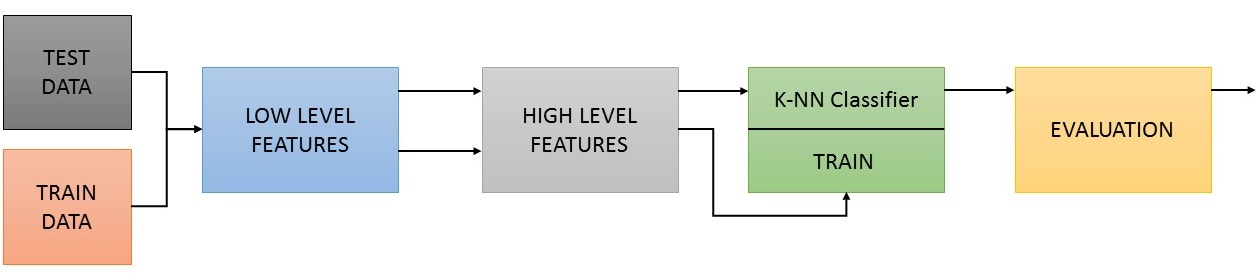
\includegraphics[width=\linewidth]{img/12.jpg}
	\label{fig:pipeline}
	\caption{Processing pipeline of test- and training-data}
		\end{center}
\end{figure}


In the following sections we discuss and document the different steps of the processing pipeline, which is shown in figure 1.

\subsection{Low-level Feature Extraction}
The low-level feature extraction individually loads the images of the test- and training-data sets, which have been created as described in section \ref{sec:data}. As soon as the $i^{th}$ image $I^{(i)}$ is loaded, the low-level featureExtraction $f_{LL}$ is applied on this image and the result, which is a feature row-vector of fixed length $L_{LL}$, is assigned to the structured data set's feature vector. The ground truth, which is retrieved from the filename of the image (denoted as class($I^{(i)}$) is stored in the structure's targets. This process is denoted as 

\begin{small}

\begin{eqnarray}
d.fv(i) & = & f_{LL}(I^{(i)}) \quad \text{with} \quad f_{LL} \in \mathbb{R}^{1 \times L_{LL}} \\
d.targets(i)& = &class((I^{(i)})
\end{eqnarray}  

\end{small}

After this is done, the data is typically stored to the hard disk as Matlab .mat files. This has the advantage of avoiding to recompute the whole pipeline while developing a certain step of the processing pipeline. Besides Classification, Lowlevel feature extraction is usually the computationally most expensive part, because it processes the largest amount of data.
\subsection{High-level Feature Extraction}
The high-level feature extraction loads the feature vectors calculate in the previous section for the test and training datasets. The same structure was followed.


\subsection{Classifier}
For classification, we use (as also in \cite{indoorScenes}) a support vector machine (SVM). The SVM is trained using the high-level features of the training data together with the class labelling retrieved from the targets, i.e. $mySVM.train(traindata.targets, traindata.fv)$. After training, $testdata.class$ is assigned the result of the prediction process $svm.predict(testdata.fv)$. 

Since SVMs are typically designed to solve two-class problems, we chose to use a LIBSVM. An implementation is available at Matlab's fileexchange\footnote{\url{http://www.csie.ntu.edu.tw/~cjlin/liblinear}}. 

\subsection{Evaluation}
\label{sec:eval}
Evaluation of the data is straight forward. It is simply evaluated, to which extent the SVM-classification lead to the correct results. That is, where the $i^{th}$ $d.class(i)$ matches the ground truth $d.targets(i)$. Formally, the recognition rate, namely the correctly classified scenes, can be computed as 
\begin{small}

\begin{equation}
	recognitionRate = \frac{1}{N} \sum_{i=1}^{N} \begin{cases}
	1 \quad \text{if} \quad d.targets(i) = d.class(i)\\
	0  \quad \text{else}
	\end{cases}
\end{equation}
\end{small}




\section{Methods}

\subsection{Low-level features}
The calculation of the low features in this case  was implemented by calculating dense SIFT descriptors:
\begin{itemize}
   \item Feature Extraction with Dense SIFT \newline
   Scale Invariant Feature Transform (SIFT) is an image descriptor for image-based matching and recognition developed by David Lowe (1999, 2004). The SIFT descriptor is invariant to translations, rotations and scaling transformations in the image domain and robust to moderate perspective transformations and illumination variations.\cite{shift} Dense SIFT used as a larger set of local image descriptors computed over a dense grid which usually provides more information than corresponding descriptors evaluated at a much sparser set of image points as described by Bosch et al. (2006, 2007). More specifically in the present case, when train and test images were loaded, they were normalised (resized to 300 x 400 or 400 x 300 depending on the image orientation). This would ensure that that we get the same number of features in every image. With our settings, the resulting DSIFT descriptors calculated were 192 per image and stored in a 3D matrix. As low level features we defined at present the DSIFT descriptors.\cite{bosch}
\end{itemize}

\subsection{High-level features}
The high level features were computed in 3 steps:
\begin{enumerate}
   \item Loading of Low level Features 
   \item Dictionary Creation by applying K-means \newline
   Using the low features in the form of a 3D matrix was achieved by mapping the 3D matrix into a 2D matrix. We defined the number of features used which were inserted for clustering. Clustering in this case is considered as encoding necessary for vector quantisation of the low features.  Clustering was performed by using K-means algorithm with the number of cluster centres being user defined. 10000 low level features were randomly selected and used.  
     
   \item Histogram Creation \newline
   At this stage the histograms for train and test images were computed. Using the Euclidean distance, we calculated the distance of the visual words to every SIFT feature  for every image. We assign every image to the cluster centre and then we get the word frequency. 
\end{enumerate}

\section{Results}
Two experiments were performed. The first using the 11 classes MIT database with varying number of cluster centres and the second with full use of the MIT database of 67 classes with varying number of cluster centres. The aim of the experiment was to observe the behaviour of  the standard average multi-class prediction accuracy regarding classification. 
\subsection{11-Classes Database}
For the 11 class problem we used different values for the cluster centres k, The values used for k and the resulting classification accuracy is shown on table 1.
\begin{table}[h]
\caption{}
\begin{tabular}{|l|l|l|l|l|l|}
\hline
Cluster Centres & 50 & 100 & 300 & 600 & 1000 \\ \hline
Accuracy & 18.27\% & 33.17\% & 49.52\% & 46.15\% & 43.75\%  \\ \hline
\end{tabular}
\end{table}

\begin{figure}[h]
      \centering
      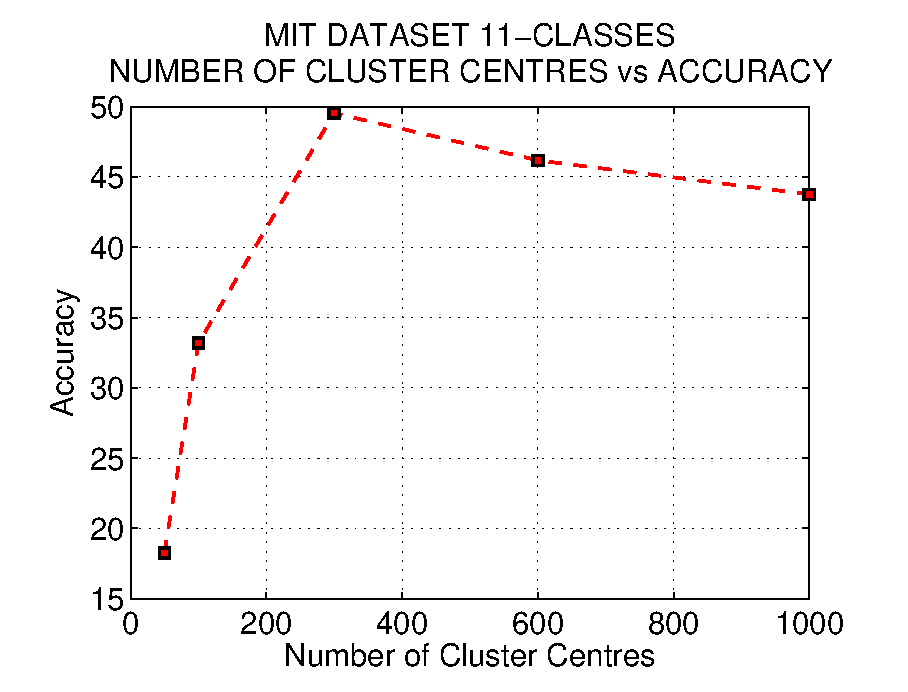
\includegraphics[width=0.7\linewidth]{img/11c.eps}
      \caption{Cluster centres vs Accuracy}
\end{figure}

From figure 2, it was observed that for the entire dataset the accuracy ranged from 18.27\% to 49.52\%. The highest accuracy of 49.52\% was observed when the number of cluster centres was 300. Above 300 cluster centres, accuracy was decreasing to 46.15\% for 600 cluster centres, and to 43.75\% for 1000 centres.


\subsection{67-Classes Database}
For the 67 class problem we used different values for the cluster centres k, The values used for k and the resulting classification accuracy used is shown on table 2.

\begin{table}[h]
\caption{}
\begin{tabular}{|l|l|l|l|}
\hline
Cluster Centres & 500 & 1000 & 1500 \\ \hline
Accuracy & 18.35\% & 17.46\% & 13.3\% \\ \hline
\end{tabular}
\end{table}
\begin{figure}[h]
      \centering
      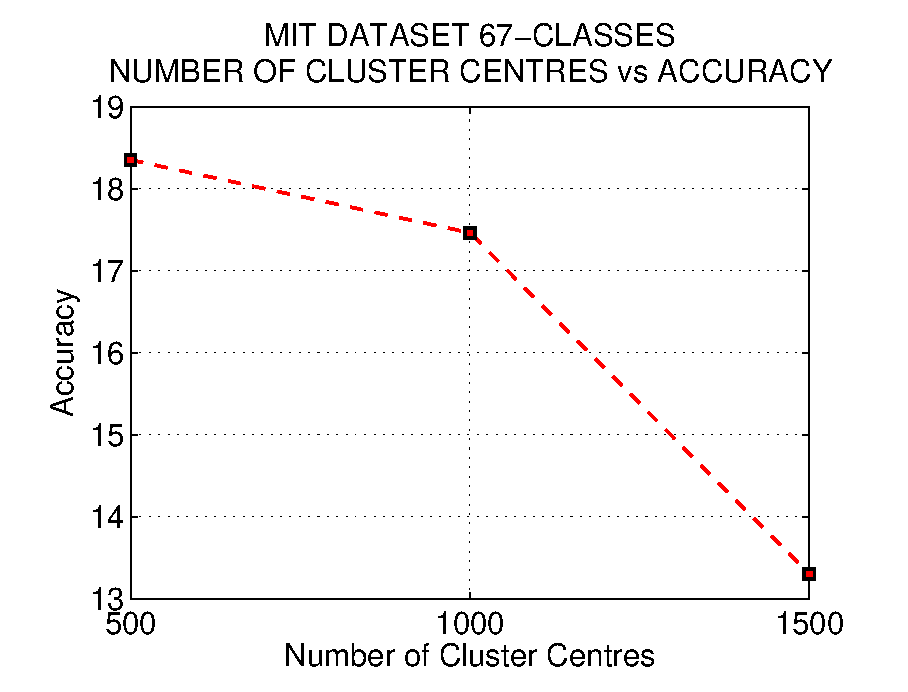
\includegraphics[width=0.8\linewidth]{img/67c.eps}
      \caption{Cluster centres vs Accuracy}
\end{figure}
From figure 3, it was observed that for the entire dataset the accuracy ranged from 13.3\% to 18.35\%. The highest accuracy of 18.35\% was observed when the number of cluster centres was 500. Above 500 cluster centres, accuracy was decreasing to 17.47\% for 1000 cluster centres and to 13.3\% for 1500 centres.  It was also observed that we achieved an accuracy of 18.35\% as our best result which is lower compared to 24.47\% that was achieved by the authors in \cite{indoorScenes}. For that comparison, we found the average value of the multi-class accuracy of 67 scene categories individually and found the mean accuracy and compared with our value. 

\section{Conclusion}
We have shown that the processes implemented and followed for Bag of visual Words (BoW) failed to produce adequate results and therefore they performed poorly.
The results from the 67  and 11 classes were not satisfying, achieving a maximum percentage of accuracy of 18.35\% and 49.52\% respectively. The low rate of accuracy of classification observed justifies that the indoor scene recognition is still an open problem. Our achieved accuracy was lower if compared to results from \cite{indoorScenes}  by 10\% in case of 67 scene categories.
{\small
\bibliographystyle{ieee}
\bibliography{egbib}
}

\end{document}
